\subsubsection{Visualization}
\label{sec:KSeMF}

To visualize the reduced \statesp\ of KS flow we will use a moving frame
to compute the first few fundamental invariants and, following the example of \CLe of \refsect{sec:CLeMF},
modify those invariants to overcome those singularities. This will help us understand what
are the invariant objects of importance in organizing the \statesp. The final goal is to choose
Poincar\'e sections that capture the dynamics but on which we can define local moving frame cross-sections, implement symmetry reduction on the Poincar\'e sections applying a moving frame on
the points of intersection of trajectories with the Poincar\'e sections and finally construct
return maps of the dynamics.

We begin by computing invariants for the ``standard action'' \refeq{eq:SO2stndrd} of $\SOn{2}$ on $\Clx{n}\cong\Rls{2n}$ which we write here as
\beq
	\left(\barr{cc} \overline{b}_k \\ \overline{c}_k\earr \right)=\left(\barr{cc}
			    			\cos(k\theta) & -\sin(k\theta)\\
						\sin(k\theta) & \cos(k\theta)\\
			   			\earr\\	
						\right) \left(\barr{cc} b_k \\ c_k\earr\right)\,,\ \ k=1,\ldots n\,.
	\label{eq:SO2stand}
\eeq
with $a_k=b_k+i c_k\,,\ b_k,c_k\in\Rls{}$.  Define the cross section by
\beq
 	K_1(a)=b_1=0\,,
\eeq
which leads to the normalization equation
\beq
	\overline{b}_1 = \cos\theta\, b_1 -\sin\theta\, c_1 = 0\,.
	\label{eq:SO2norm}
\eeq
The obvious solution is $\theta=\tan^{-1}\frac{b_1}{c_1}$, but we prefer to use the moving frame
\beq
	\theta=
\eeq
which is a solution of \refeq{eq:SO2norm} and, when substituted back in \refeq{eq:SO2stand} results in invariants that do not depend on the sign of $b_1$.

\ES{The Gr\"{o}bner basis methods usually perform poorly as $n$ becomes larger than six. On a 1GHz Pentium III processor the fundamental invariants for $n=16$, for the cross
section $b_1=0$, were computed in approximately 130s. Most importantly the time was mostly
spend in simplification of expressions.
If one only wants to project equivariant dynamics on the \reducedsp\ then the moving frame method,
through its geometric interpretation, can be used to perform the projection without explicit knowledge of the fundamental invariants.
This idea will become clear in the example of \reducedsp\ projection
for \CLe.}
The fundamental invariants for \SOn{2} acting as in \refeq{eq:SO2stand} with
$n=6$ calculated with the method of moving frames are listed in \reftab{tab:SO2n6}. Note another advantage of the method: no syzygies are present.

\begin{table}[t]
\[
\begin{array}{ll}
  u_1=r_1=\sqrt{b_1^2+c_1^2}&  \\ u_3=\frac{b_2 \left(b_1^2-c_1^2\right)+2 b_1 c_1 c_2}{r_1^2}&u_4=\frac{-2
b_1 b_2 c_1+\left(b_1^2-c_1^2\right) c_2}{r_1^2}\\ u_5=\frac{b_1 b_3 \left(b_1^2-3 c_1^2\right)-c_1 \left(-3
b_1^2+c_1^2\right) c_3}{r_1^3}&u_6=\frac{-3 b_1^2 b_3 c_1+b_3 c_1^3+b_1^3 c_3-3 b_1 c_1^2 c_3}{r_1^3}\\ u_7=\frac{b_4
\left(b_1^4-6 b_1^2 c_1^2+c_1^4\right)+4 b_1 c_1 \left(b_1^2-c_1^2\right) c_4}{r_1^4}&u_8=\frac{4 b_1
b_4 c_1 \left(-b_1^2+c_1^2\right)+\left(b_1^4-6 b_1^2 c_1^2+c_1^4\right) c_4}{r_1^4}\\ u_9=\frac{b_1
b_5 \left(b_1^4-10 b_1^2 c_1^2+5 c_1^4\right)+c_1 \left(5 b_1^4-10 b_1^2 c_1^2+c_1^4\right) c_5}{r_1^5}&u_{10}=\frac{-b_5
c_1 \left(5 b_1^4-10 b_1^2 c_1^2+c_1^4\right)+b_1 \left(b_1^4-10 b_1^2 c_1^2+5 c_1^4\right) c_5}{r_1^5}\\ u_{11}=\frac{b_6
\left(b_1^6-15 b_1^4 c_1^2+15 b_1^2 c_1^4-c_1^6\right)+2 b_1 c_1 \left(3 b_1^4-10 b_1^2 c_1^2+3 c_1^4\right) c_6}{r_1^6}&u_{12}=\frac{-2
b_1 b_6 c_1 \left(3 b_1^4-10 b_1^2 c_1^2+3 c_1^4\right)+\left(b_1^6-15 b_1^4 c_1^2+15 b_1^2 c_1^4-c_1^6\right) c_6}{r_1^6}\\
\end{array}
\]
\caption[Fundamental invariants for SO(2), n=6.]
{Fundamental invariants for the standard action of \SOn{2} on \Rls{6}}
\label{tab:SO2n6}
\end{table}

The first few fundamental invariants for the action
\refeq{eq:shiftF} of $\SOn{2}\subset\On{2}$ on the \statesp\
of \KSe\ have been tabulated in \reftab{tab:SO2n6}. The obvious
singularity at $b_1=c_1=0$ can be corrected by substituting
$r_1$ with $r=\sum_{i=1}^3 (b_i^2+c_i^2)$ in the denominators.
The reason for using only the first three mode magnitudes is
that this choice is enough to prevent the denominator from
vanishing at one of the three equilibria $E_i$, $i=1\ldots3$.
With this modification one has to note that the invariants of
\reftab{tab:SO2n6} vanish at \EQB{2} and \EQB{3}. In principle
this is not a problem since we want to carry out reduction in
the principal stratum. In practice this causes two important
equilibria to be mapped to the origin and leads to \statesp\
portraits as in \reffig{fig:ksSO2eqbTo0}. The neighborhood of
\EQB{2} and \EQB{3} which is where we would like to get some
intuition about the behavior of \rpo s, has been squeezed into
a cone-shaped surface\ES{Write this in the text properly: We
could overcome this by using the sixth fourier component to
setup the moving frame but then the expressions we get after
substitution cannot be simplified and we are left with the
denominators. We can use the sixth mode to setup the moving
frame in the final version, after we find Poincare sections.}.

%%%%%%%%%%%%%%%%%%%%%%%%%%%%%%%%%%%%%%%%%%%%%%%%%%%%%%%%%%%%%%%%%%
\begin{figure}[t]
\begin{center}
  (\textit{a})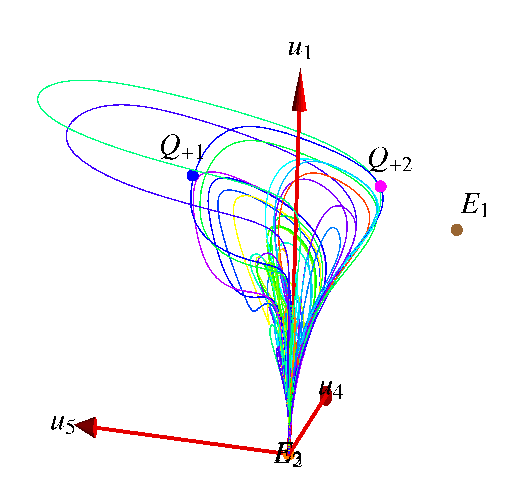
\includegraphics[width=0.4\textwidth]{../figs/ksSO2inv145eqbTo0.eps}
\end{center}
\caption[KSe SO(2) reduced phase space with modified invariants.]
   {\Statesp\ portrait of $L=22$ \KS\ dynamics projected to
   invariants given in \reftab{tab:SO2n6}. The trajectories
   shown are 20 short \rpo s. }
\label{fig:ksSO2eqbTo0}
\end{figure}
%%%%%%%%%%%%%%%%%%%%%%%%%%%%%%%%%%%%%%%%%%%%%%%%%%%%%%%%%%%%%%%%

To overcome this problem we modify the invariants of  \reftab{tab:SO2n6} as follows. We observe that the invariants come as either symmetric or antisymmetric under the action of $\Dn{1}\subset\On{2}$. We modify the symmetric invariants by adding a term $\sqrt{b_i^2+c_i^2}$ where $i$ the corresponding irreducible subspace  (Fourier mode). The new invariants are listed in \reftab{tab:SO2n6modif}.

\begin{table}
\begin{small}
\begin{eqnarray*}
  u_1=r_1 &=&\sqrt{b_1^2+c_1^2}\\
  u_3 &=&\frac{b_2 \left(b_1^2-c_1^2\right)+2 b_1 c_1 c_2}{r^2}\\
  u_4 &=&\sqrt{b_2^2+c_2^2}+\frac{-2
b_1 b_2 c_1+\left(b_1^2-c_1^2\right) c_2}{r^2}\\
  u_5 &=&\sqrt{b_3^2+c_3^2}+\frac{b_1 b_3 \left(b_1^2-3 c_1^2\right)-c_1 \left(-3
b_1^2+c_1^2\right) c_3}{r^3}\\
  u_6 &=&\frac{-3 b_1^2 b_3 c_1+b_3 c_1^3+b_1^3 c_3-3 b_1 c_1^2 c_3}{r^3}\\
  u_7 &=&\frac{b_4
\left(b_1^4-6 b_1^2 c_1^2+c_1^4\right)+4 b_1 c_1 \left(b_1^2-c_1^2\right) c_4}{r^4}\\
  u_8 &=&\sqrt{b_4^2+c_4^2}+\frac{4 b_1
b_4 c_1 \left(-b_1^2+c_1^2\right)+\left(b_1^4-6 b_1^2 c_1^2+c_1^4\right) c_4}{r^4}\\
  u_9 &=&\sqrt{b_5^2+c_5^2}+\frac{b_1
b_5 \left(b_1^4-10 b_1^2 c_1^2+5 c_1^4\right)+c_1 \left(5 b_1^4-10 b_1^2 c_1^2+c_1^4\right) c_5}{r^5}\\
  u_{10} &=&\frac{-b_5
c_1 \left(5 b_1^4-10 b_1^2 c_1^2+c_1^4\right)+b_1 \left(b_1^4-10 b_1^2 c_1^2+5 c_1^4\right) c_5}{r^5}\\
  u_{11} &=&\frac{b_6
\left(b_1^6-15 b_1^4 c_1^2+15 b_1^2 c_1^4-c_1^6\right)+2 b_1 c_1 \left(3 b_1^4-10 b_1^2 c_1^2+3 c_1^4\right) c_6}{r^6} \\
  u_{12} &=&\sqrt{b_6^2+c_6^2}+\frac{-2
b_1 b_6 c_1 \left(3 b_1^4-10 b_1^2 c_1^2+3 c_1^4\right)+\left(b_1^6-15 b_1^4 c_1^2+15 b_1^2 c_1^4-c_1^6\right) c_6}{r^6}
\end{eqnarray*}
\caption[Modified invariants for SO(2), n=6.]{Modified invariants for the standard action of \SOn{2} on \Rls{6}}
\label{tab:SO2n6modif}
\end{small}
\end{table}

\Statesp\ projections on those invariants are shown in
\reffig{fig:SO2inv}\ES{Sophia says: Do not scrible-scrable!}.
\ES{Those projections make me feel desperate. My only hope is
that the unstable manifolds of the relative equilibria and the
unstable manifolds of the antisymmetric equilibria that are not
restricted in the antisymmetric subspace (and we haven't payed
any attention to) will play some role in organizing this mess.}
A trajectory on the unstable manifold of $\REQB{-1}$ has been
plotted along with a few of the shortest orbits. We observe
that even though the neighborhood of \REQB{\pm 1} is not visited
by the turbulent dynamics or the \rpo s, the unstable manifolds
of \REQB{\pm1} play an important role in organizing the flow.


%%%%%%%%%%%%%%%%%%%%%%%%%%%%%%%%%%%%%%%%%%%%%%%%%%%%%%%%%%%%%%%%%%
\begin{figure}[t]
\begin{center}
  (\textit{a})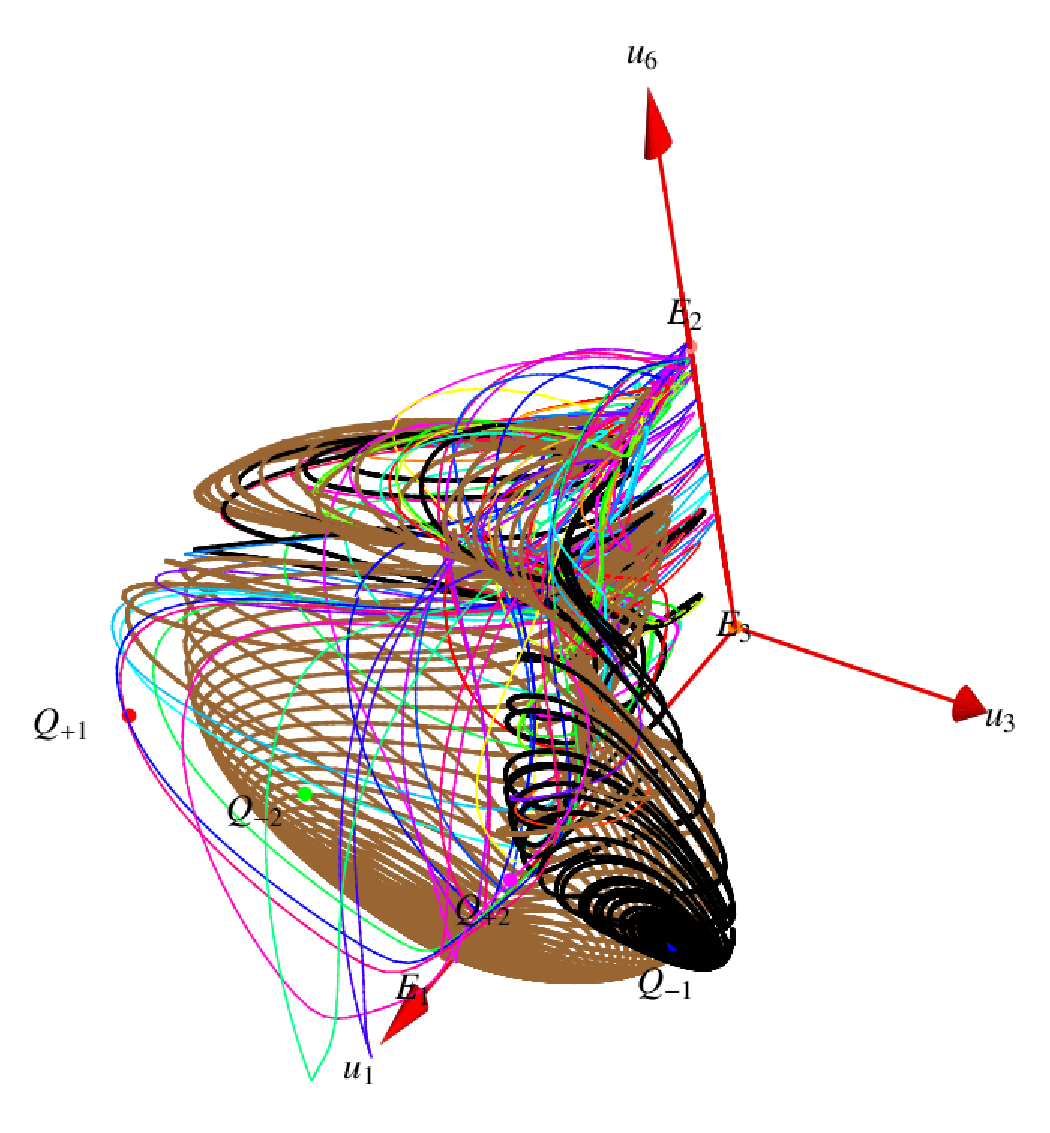
\includegraphics[width=0.35\textwidth]{../figs/ksSO2inv134.eps}
~~~~(\textit{b})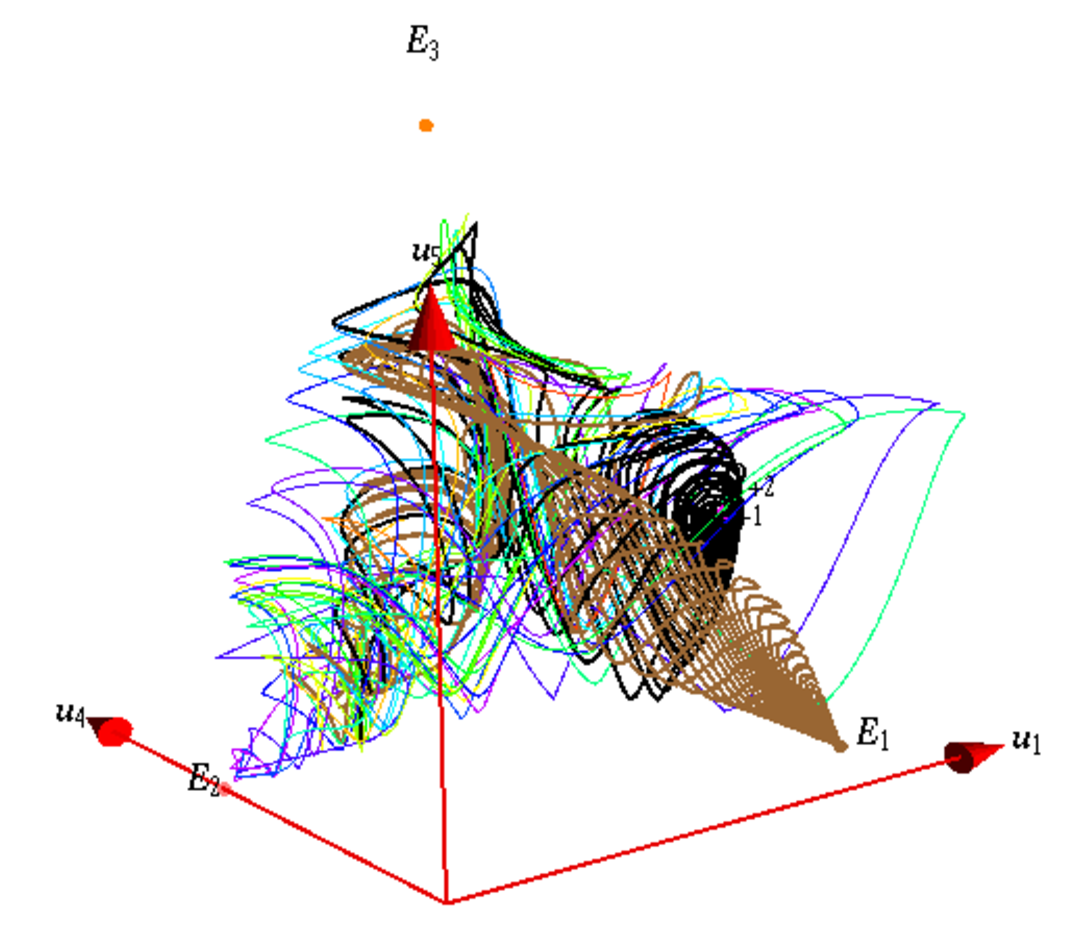
\includegraphics[width=0.35\textwidth]{../figs/ksSO2inv145.eps}
\end{center}
\caption[KSe SO(2) reduced phase space with
         second set of modified invariants.]
{Two different projections of L=22 \KS\ dynamics on invariants
given in \reftab{tab:SO2n6modif}. Shown are 20
short \rpo s. A trajectory on the unstable manifold of
$\REQB{1}$ is shown in black.}
\label{fig:SO2inv}
\end{figure}
%%%%%%%%%%%%%%%%%%%%%%%%%%%%%%%%%%%%%%%%%%%%%%%%%%%%%%%%%%%%%%%%
